\documentclass[11pt]{article}

\usepackage{fullpage}
\usepackage{amsmath, amssymb, bm, cite, epsfig, psfrag}
\usepackage{graphicx}
\usepackage{float}
\usepackage{amsthm}
\usepackage{amsfonts}
\usepackage{listings}
\usepackage{cite}
\usepackage{hyperref}
\usepackage{tikz}
\usepackage{enumerate}
\usepackage{listings}
\usepackage{mathtools}
\lstloadlanguages{Python}
\usetikzlibrary{shapes,arrows,positioning}

\DeclareFixedFont{\ttb}{T1}{txtt}{bx}{n}{9} % for bold
\DeclareFixedFont{\ttm}{T1}{txtt}{m}{n}{9}  % for normal
% Defining colors
\usepackage{color}
\definecolor{deepblue}{rgb}{0,0,0.5}
\definecolor{deepred}{rgb}{0.6,0,0}
\definecolor{deepgreen}{rgb}{0,0.5,0}
\definecolor{backcolour}{rgb}{0.95,0.95,0.92}

\def\del{\partial}
\def\ds{\displaystyle}
\def\ts{\textstyle}
\def\beq{\begin{equation}}
\def\eeq{\end{equation}}
\def\beqa{\begin{eqnarray}}
\def\eeqa{\end{eqnarray}}
\def\beqan{\begin{eqnarray*}}
\def\eeqan{\end{eqnarray*}}
\def\nn{\nonumber}
\def\binomial{\mathop{\mathrm{binomial}}}
\def\half{{\ts\frac{1}{2}}}
\def\Half{{\frac{1}{2}}}
\def\N{{\mathbb{N}}}
\def\Z{{\mathbb{Z}}}
\def\Q{{\mathbb{Q}}}
\def\R{{\mathbb{R}}}
\def\C{{\mathbb{C}}}
\def\argmin{\mathop{\mathrm{arg\,min}}}
\def\argmax{\mathop{\mathrm{arg\,max}}}
\def\diag{\mathop{\mathrm{diag}}}
\def\x{\times}
\def\limn{\lim_{n \rightarrow \infty}}
\def\liminfn{\liminf_{n \rightarrow \infty}}
\def\limsupn{\limsup_{n \rightarrow \infty}}
\def\GV{Guo and Verd{\'u}}
\def\MID{\,|\,}
\def\MIDD{\,;\,}

\newtheorem{proposition}{Proposition}
\newtheorem{definition}{Definition}
\newtheorem{theorem}{Theorem}
\newtheorem{lemma}{Lemma}
\newtheorem{corollary}{Corollary}
\newtheorem{assumption}{Assumption}
\newtheorem{claim}{Claim}
\def\qed{\mbox{} \hfill $\Box$}
\setlength{\unitlength}{1mm}

\def\bhat{\widehat{b}}
\def\ehat{\widehat{e}}
\def\phat{\widehat{p}}
\def\qhat{\widehat{q}}
\def\rhat{\widehat{r}}
\def\shat{\widehat{s}}
\def\uhat{\widehat{u}}
\def\ubar{\overline{u}}
\def\vhat{\widehat{v}}
\def\xhat{\widehat{x}}
\def\xbar{\overline{x}}
\def\zhat{\widehat{z}}
\def\zbar{\overline{z}}
\def\la{\leftarrow}
\def\ra{\rightarrow}
\def\MSE{\mbox{\small \sffamily MSE}}
\def\SNR{\mbox{\small \sffamily SNR}}
\def\SINR{\mbox{\small \sffamily SINR}}
\def\arr{\rightarrow}
\def\Exp{\mathbb{E}}
\def\var{\mbox{var}}
\def\Tr{\mbox{Tr}}
\def\tm1{t\! - \! 1}
\def\tp1{t\! + \! 1}
\def\Tm1{T\! - \! 1}
\def\Tp1{T\! + \! 1}


\def\Xset{{\cal X}}

\newcommand{\one}{\mathbf{1}}
\newcommand{\abf}{\mathbf{a}}
\newcommand{\bbf}{\mathbf{b}}
\newcommand{\dbf}{\mathbf{d}}
\newcommand{\ebf}{\mathbf{e}}
\newcommand{\gbf}{\mathbf{g}}
\newcommand{\hbf}{\mathbf{h}}
\newcommand{\pbf}{\mathbf{p}}
\newcommand{\pbfhat}{\widehat{\mathbf{p}}}
\newcommand{\qbf}{\mathbf{q}}
\newcommand{\qbfhat}{\widehat{\mathbf{q}}}
\newcommand{\rbf}{\mathbf{r}}
\newcommand{\rbfhat}{\widehat{\mathbf{r}}}
\newcommand{\sbf}{\mathbf{s}}
\newcommand{\sbfhat}{\widehat{\mathbf{s}}}
\newcommand{\ubf}{\mathbf{u}}
\newcommand{\ubfhat}{\widehat{\mathbf{u}}}
\newcommand{\utildebf}{\tilde{\mathbf{u}}}
\newcommand{\vbf}{\mathbf{v}}
\newcommand{\vbfhat}{\widehat{\mathbf{v}}}
\newcommand{\wbf}{\mathbf{w}}
\newcommand{\wbfhat}{\widehat{\mathbf{w}}}
\newcommand{\xbf}{\mathbf{x}}
\newcommand{\xbfhat}{\widehat{\mathbf{x}}}
\newcommand{\xbfbar}{\overline{\mathbf{x}}}
\newcommand{\ybf}{\mathbf{y}}
\newcommand{\zbf}{\mathbf{z}}
\newcommand{\zbfbar}{\overline{\mathbf{z}}}
\newcommand{\zbfhat}{\widehat{\mathbf{z}}}
\newcommand{\Ahat}{\widehat{A}}
\newcommand{\Abf}{\mathbf{A}}
\newcommand{\Bbf}{\mathbf{B}}
\newcommand{\Cbf}{\mathbf{C}}
\newcommand{\Bbfhat}{\widehat{\mathbf{B}}}
\newcommand{\Dbf}{\mathbf{D}}
\newcommand{\Gbf}{\mathbf{G}}
\newcommand{\Hbf}{\mathbf{H}}
\newcommand{\Ibf}{\mathbf{I}}
\newcommand{\Kbf}{\mathbf{K}}
\newcommand{\Pbf}{\mathbf{P}}
\newcommand{\Phat}{\widehat{P}}
\newcommand{\Qbf}{\mathbf{Q}}
\newcommand{\Rbf}{\mathbf{R}}
\newcommand{\Rhat}{\widehat{R}}
\newcommand{\Sbf}{\mathbf{S}}
\newcommand{\Ubf}{\mathbf{U}}
\newcommand{\Vbf}{\mathbf{V}}
\newcommand{\Wbf}{\mathbf{W}}
\newcommand{\Xhat}{\widehat{X}}
\newcommand{\Xbf}{\mathbf{X}}
\newcommand{\Ybf}{\mathbf{Y}}
\newcommand{\Zbf}{\mathbf{Z}}
\newcommand{\Zhat}{\widehat{Z}}
\newcommand{\Zbfhat}{\widehat{\mathbf{Z}}}
\def\alphabf{{\boldsymbol \alpha}}
\def\betabf{{\boldsymbol \beta}}
\def\betabfhat{{\widehat{\bm{\beta}}}}
\def\epsilonbf{{\boldsymbol \epsilon}}
\def\mubf{{\boldsymbol \mu}}
\def\lambdabf{{\boldsymbol \lambda}}
\def\etabf{{\boldsymbol \eta}}
\def\xibf{{\boldsymbol \xi}}
\def\taubf{{\boldsymbol \tau}}
\def\sigmahat{{\widehat{\sigma}}}
\def\thetabf{{\bm{\theta}}}
\def\thetabfhat{{\widehat{\bm{\theta}}}}
\def\thetahat{{\widehat{\theta}}}
\def\mubar{\overline{\mu}}
\def\muavg{\mu}
\def\sigbf{\bm{\sigma}}
\def\etal{\emph{et al.}}
\def\Ggothic{\mathfrak{G}}
\def\Pset{{\mathcal P}}
\newcommand{\bigCond}[2]{\bigl({#1} \!\bigm\vert\! {#2} \bigr)}
\newcommand{\BigCond}[2]{\Bigl({#1} \!\Bigm\vert\! {#2} \Bigr)}
\newcommand{\tran}{^{\text{\sf T}}}
\newcommand{\herm}{^{\text{\sf H}}}
\newcommand{\bkt}[1]{{\langle #1 \rangle}}
\def\Norm{{\mathcal N}}
\newcommand{\vmult}{.}
\newcommand{\vdiv}{./}


% Python style for highlighting
\newcommand\pythonstyle{\lstset{
language=Python,
backgroundcolor=\color{backcolour},
commentstyle=\color{deepgreen},
basicstyle=\ttm,
otherkeywords={self},             % Add keywords here
keywordstyle=\ttb\color{deepblue},
emph={MyClass,__init__},          % Custom highlighting
emphstyle=\ttb\color{deepred},    % Custom highlighting style
stringstyle=\color{deepgreen},
%frame=tb,                         % Any extra options here
showstringspaces=false            %
}}

% Python environment
\lstnewenvironment{python}[1][]
{
\pythonstyle
\lstset{#1}
}
{}

% Python for external files
\newcommand\pythonexternal[2][]{{
\pythonstyle
\lstinputlisting[#1]{#2}}}

% Python for inline
\newcommand\pycode[1]{{\pythonstyle\lstinline!#1!}}

\begin{document}

\title{Introduction to Machine Learning\\
$K$-means and Clustering Problems\\Solutions}
\author{Prof. Sundeep Rangan}
\date{}

\maketitle

\section*{Problem 1}

You are given five data samples:

\begin{center}
\begin{tabular}{|c|c|c|c|c|c|}  \hline
$i$ & 1 & 2 & 3 & 4 & 5 \\ \hline
$x_{i1}$ & 0 & 1 & 0 & 2 & 2 \\ \hline
$x_{i2}$ & 0 & 0 & 1 & 2 & 3 \\ \hline
\end{tabular}
\end{center}

\subsection*{(a) Draw the five points.}

\begin{figure}[h]
\centering
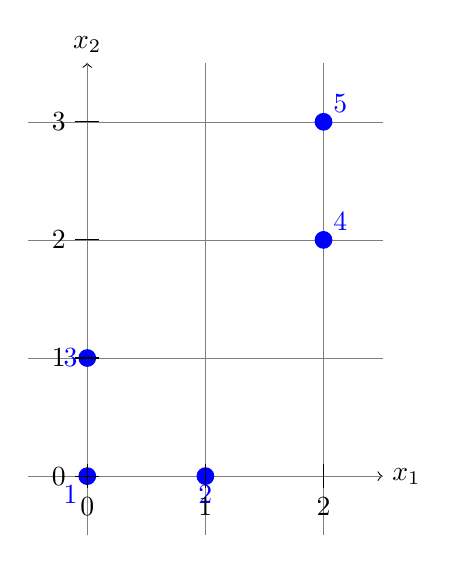
\begin{tikzpicture}[scale=1.5]
% Draw axes
\draw[->] (-0.5,0) -- (2.5,0) node[right] {$x_1$};
\draw[->] (0,-0.5) -- (0,3.5) node[above] {$x_2$};

% Draw grid
\draw[gray, very thin] (-0.5,-0.5) grid (2.5,3.5);

% Draw points
\filldraw[blue] (0,0) circle (2pt) node[below left] {1};
\filldraw[blue] (1,0) circle (2pt) node[below] {2};
\filldraw[blue] (0,1) circle (2pt) node[left] {3};
\filldraw[blue] (2,2) circle (2pt) node[above right] {4};
\filldraw[blue] (2,3) circle (2pt) node[above right] {5};

% Label axes
\foreach \x in {0,1,2}
    \draw (\x,0.1) -- (\x,-0.1) node[below] {\x};
\foreach \y in {0,1,2,3}
    \draw (0.1,\y) -- (-0.1,\y) node[left] {\y};
\end{tikzpicture}
\caption{Plot of the five data points} \label{fig:points}
\end{figure}

\subsection*{(b) Starting with $K=2$ cluster centers at $(0,0)$ and $(1,0)$, what are the cluster assignments and new cluster centers after one iteration of $K$-means?}

\textbf{Step 1: Assignment Step}

For each point, compute the squared Euclidean distance to both cluster centers and assign to the nearest center.

\begin{itemize}
\item \textbf{Point 1} $(0,0)$:
  \begin{itemize}
  \item Distance to center 1 $(0,0)$: $d^2 = (0-0)^2 + (0-0)^2 = 0$
  \item Distance to center 2 $(1,0)$: $d^2 = (0-1)^2 + (0-0)^2 = 1$
  \item Assignment: \textbf{Cluster 1}
  \end{itemize}

\item \textbf{Point 2} $(1,0)$:
  \begin{itemize}
  \item Distance to center 1 $(0,0)$: $d^2 = (1-0)^2 + (0-0)^2 = 1$
  \item Distance to center 2 $(1,0)$: $d^2 = (1-1)^2 + (0-0)^2 = 0$
  \item Assignment: \textbf{Cluster 2}
  \end{itemize}

\item \textbf{Point 3} $(0,1)$:
  \begin{itemize}
  \item Distance to center 1 $(0,0)$: $d^2 = (0-0)^2 + (1-0)^2 = 1$
  \item Distance to center 2 $(1,0)$: $d^2 = (0-1)^2 + (1-0)^2 = 2$
  \item Assignment: \textbf{Cluster 1}
  \end{itemize}

\item \textbf{Point 4} $(2,2)$:
  \begin{itemize}
  \item Distance to center 1 $(0,0)$: $d^2 = (2-0)^2 + (2-0)^2 = 8$
  \item Distance to center 2 $(1,0)$: $d^2 = (2-1)^2 + (2-0)^2 = 5$
  \item Assignment: \textbf{Cluster 2}
  \end{itemize}

\item \textbf{Point 5} $(2,3)$:
  \begin{itemize}
  \item Distance to center 1 $(0,0)$: $d^2 = (2-0)^2 + (3-0)^2 = 13$
  \item Distance to center 2 $(1,0)$: $d^2 = (2-1)^2 + (3-0)^2 = 10$
  \item Assignment: \textbf{Cluster 2}
  \end{itemize}
\end{itemize}

\textbf{Cluster assignments:}
\begin{itemize}
\item \textbf{Cluster 1}: Points 1 and 3: $\{(0,0), (0,1)\}$
\item \textbf{Cluster 2}: Points 2, 4, and 5: $\{(1,0), (2,2), (2,3)\}$
\end{itemize}

\textbf{Step 2: Update Step}

Compute new cluster centers as the mean of assigned points:

\begin{itemize}
\item \textbf{New Center 1}: 
  \[
  \mu_1 = \frac{(0,0) + (0,1)}{2} = \left(\frac{0+0}{2}, \frac{0+1}{2}\right) = (0, 0.5)
  \]

\item \textbf{New Center 2}: 
  \[
  \mu_2 = \frac{(1,0) + (2,2) + (2,3)}{3} = \left(\frac{1+2+2}{3}, \frac{0+2+3}{3}\right) = \left(\frac{5}{3}, \frac{5}{3}\right) \approx (1.67, 1.67)
  \]
\end{itemize}

\textbf{Answer:} After one iteration:
\begin{itemize}
\item \textbf{Cluster assignments}: Cluster 1: $\{1, 3\}$, Cluster 2: $\{2, 4, 5\}$
\item \textbf{New cluster centers}: $\mu_1 = (0, 0.5)$, $\mu_2 = (5/3, 5/3) \approx (1.67, 1.67)$
\end{itemize}

\newpage

\section*{Problem 2}

\emph{$K$-means for outlier detection.} Write a function for outlier detection:

\subsection*{Solution}

\begin{python}
def outlier_detect(Xtr, Xts, nc, t):
    """
    Detect outliers using K-means clustering.
    
    Parameters:
    Xtr: Training data (N_tr x D matrix)
    Xts: Test data (N_ts x D matrix)
    nc: Number of clusters
    t: Distance threshold
    
    Returns:
    outlier: Binary array (N_ts x 1), 1 if outlier, 0 otherwise
    """
    from sklearn.cluster import KMeans
    import numpy as np
    
    # Perform K-means on training data
    km = KMeans(n_clusters=nc)
    km.fit(Xtr)
    
    # Get cluster centers (nc x D matrix)
    centers = km.cluster_centers_  # Shape: (nc, D)
    
    # Compute distances from each test point to all cluster centers
    # Xts: (N_ts, D), centers: (nc, D)
    # We want: distances[i, j] = ||Xts[i] - centers[j]||^2
    
    # Using broadcasting:
    # Xts[:, None, :] has shape (N_ts, 1, D)
    # centers[None, :, :] has shape (1, nc, D)
    # Difference has shape (N_ts, nc, D)
    diff = Xts[:, None, :] - centers[None, :, :]
    distances_sq = np.sum(diff**2, axis=2)  # Shape: (N_ts, nc)
    
    # Find minimum distance from each test point to any cluster center
    min_distances = np.sqrt(np.min(distances_sq, axis=1))  # Shape: (N_ts,)
    
    # Mark as outlier if distance > threshold
    outlier = (min_distances > t).astype(int)
    
    return outlier
\end{python}

\textbf{Explanation:}
\begin{itemize}
\item We use broadcasting to compute all pairwise distances efficiently without loops
\item \pycode{Xts[:, None, :]} reshapes to $(N_{ts}, 1, D)$ for broadcasting
\item \pycode{centers[None, :, :]} reshapes to $(1, nc, D)$ for broadcasting
\item The difference gives us $(N_{ts}, nc, D)$, then we sum over the last axis to get squared distances
\item We find the minimum distance for each test point and compare to threshold
\end{itemize}

\newpage

\section*{Problem 3}

\emph{Initialization.} Write a few lines of python code to initialize $K$-means by selecting $K$ random samples of the training data as the cluster centers. Make sure you do not pick the same sample twice.

\subsection*{Solution}

\begin{python}
import numpy as np

# Method 1: Using np.random.choice (recommended)
n = Xtr.shape[0]  # Number of training samples
indices = np.random.choice(n, size=K, replace=False)
mu_init = Xtr[indices, :]

# Method 2: Using random permutation
indices = np.random.permutation(n)[:K]
mu_init = Xtr[indices, :]

# Method 3: Manual approach (less efficient but clear)
indices = []
while len(indices) < K:
    idx = np.random.randint(0, n)
    if idx not in indices:
        indices.append(idx)
mu_init = Xtr[indices, :]
\end{python}

\textbf{Explanation:}
\begin{itemize}
\item \pycode{np.random.choice(n, size=K, replace=False)} selects $K$ unique indices from $[0, n)$
\item \pycode{replace=False} ensures no duplicates
\item \pycode{Xtr[indices, :]} extracts the corresponding rows from the training data
\item Method 1 is the most efficient and Pythonic approach
\end{itemize}

\newpage

\section*{Problem 4}

\emph{Clustering as pre-processing.} Suppose we want to cluster data and then fit a linear model in each cluster. You are given training data \pycode{Xtr,ytr} and test data \pycode{Xts,yts} for a regression problem. Write code to do the following:
\begin{itemize}
  \item Perform $K$-means clustering on the training data \pycode{Xtr} with a given number \pycode{nc} clusters;
  \item In each cluster in the training data, fit a linear model.
  \item Compute the predicted outputs \pycode{yhat_ts} and mean squared error of the model on the test data.
\end{itemize}

\subsection*{Solution}

\begin{python}
from sklearn.cluster import KMeans
from sklearn.linear_model import LinearRegression
import numpy as np

# Perform K-means clustering on training data
km = KMeans(n_clusters=nc)
km.fit(Xtr)

# Get cluster assignments for training data
cluster_train = km.predict(Xtr)  # Shape: (N_tr,)

# Get cluster assignments for test data
cluster_test = km.predict(Xts)  # Shape: (N_ts,)

# Initialize list to store regression models for each cluster
regressors = [LinearRegression() for _ in range(nc)]

# Fit a linear model in each cluster
for k in range(nc):
    # Find training samples in cluster k
    mask_train = (cluster_train == k)
    Xtr_k = Xtr[mask_train, :]
    ytr_k = ytr[mask_train]
    
    # Fit linear model for cluster k
    if Xtr_k.shape[0] > 0:  # Check if cluster has samples
        regressors[k].fit(Xtr_k, ytr_k)

# Predict on test data
yhat_ts = np.zeros(yts.shape)
for k in range(nc):
    # Find test samples in cluster k
    mask_test = (cluster_test == k)
    if np.any(mask_test) and Xtr[cluster_train == k].shape[0] > 0:
        # Predict using the model for cluster k
        yhat_ts[mask_test] = regressors[k].predict(Xts[mask_test, :])

# Compute mean squared error
mse = np.mean((yts - yhat_ts)**2)
\end{python}

\textbf{Explanation:}
\begin{itemize}
\item We create a list of \pycode{LinearRegression} objects, one for each cluster
\item For each cluster, we extract the training samples belonging to that cluster and fit a linear model
\item For prediction, we assign each test sample to its cluster and use the corresponding regression model
\item We handle edge cases where a cluster might have no training samples
\end{itemize}

\newpage

\section*{Problem 5}

Figure \ref{fig:samples} shows a set of samples to be clustered. Show the results from K-means algorithm in successive iterations, starting with the initial centroids indicated in the figure. You can do nearest neighbor partition and centroid update approximately by ``eyeballing''.

\begin{figure}[h]
\centering
\includegraphics[width=0.5\columnwidth]{samples.png}
\caption{The set of samples to be clustered} \label{fig:samples}
\end{figure}

\subsection*{Solution}

\textbf{Note:} Without access to the actual figure, I'll provide a general approach for solving this problem:

\begin{enumerate}
\item \textbf{Initialization}: Identify the initial centroids marked in Figure~\ref{fig:samples}

\item \textbf{Iteration 1 - Assignment Step}:
  \begin{itemize}
  \item For each data point, compute the distance to all centroids
  \item Assign each point to the nearest centroid
  \item Draw the Voronoi diagram (partition boundaries) showing which points belong to which cluster
  \end{itemize}

\item \textbf{Iteration 1 - Update Step}:
  \begin{itemize}
  \item Compute the new centroid for each cluster as the mean of all points assigned to it
  \item Mark the new centroid positions
  \end{itemize}

\item \textbf{Iteration 2}: Repeat the assignment and update steps with the new centroids

\item \textbf{Continue} until convergence (centroids no longer change significantly)
\end{enumerate}

\textbf{General Procedure:}
\begin{itemize}
\item Draw the current partition boundaries (perpendicular bisectors between centroids)
\item Color-code points by their cluster assignment
\item Compute and mark new centroids
\item Repeat until the algorithm converges
\end{itemize}

\newpage

\section*{Problem 6}

Suppose you have conducted a clustering analysis for a dataset with each sample described by $D$ features, and you used K-means algorithm to derive $K$ clusters and determined the cluster model parameters (including the centroids of the $K$ clusters). Given a test dataset containing $N$ samples, you want to classify each sample into one of the cluster using the nearest neighbor rule. How many computations are needed? For simplicity, for this and all following problems, only count multiplications (consider the square operation as multiplication).

\subsection*{Solution}

For each test sample, we need to:
\begin{enumerate}
\item Compute the squared distance to each of the $K$ cluster centers
\item Find the minimum distance
\end{enumerate}

\textbf{For one test sample:}
\begin{itemize}
\item Distance to one cluster center: $D$ subtractions + $D$ multiplications (squaring) + $(D-1)$ additions
\item Since we only count multiplications: $D$ multiplications per cluster center
\item For $K$ cluster centers: $K \times D$ multiplications
\item Finding the minimum: negligible (comparisons, not multiplications)
\end{itemize}

\textbf{For $N$ test samples:}
\[
\text{Total multiplications} = N \times K \times D
\]

\textbf{Answer:} $NKD$ multiplications

\newpage

\section*{Problem 7}

Suppose you are given $N$ samples each described by $D$ features, and you are asked to cluster them into $K$ clusters using the K-means algorithm. Suppose you run the K-means iteration $T$ times. How many computations are needed?

\subsection*{Solution}

Each iteration of K-means consists of two steps:

\textbf{Step 1: Assignment Step}
\begin{itemize}
\item For each of $N$ samples, compute distance to $K$ cluster centers
\item Each distance computation: $D$ multiplications (for squared differences)
\item Total: $N \times K \times D$ multiplications per iteration
\end{itemize}

\textbf{Step 2: Update Step}
\begin{itemize}
\item For each of $K$ clusters, compute the mean of assigned points
\item For cluster $k$ with $n_k$ points:
  \begin{itemize}
  \item Sum $n_k$ vectors of dimension $D$: $n_k \times D$ additions (not counted)
  \item Divide by $n_k$: $D$ divisions (not counted as multiplications)
  \item No multiplications needed for this step
  \end{itemize}
\end{itemize}

\textbf{Total for $T$ iterations:}
\[
\text{Total multiplications} = T \times N \times K \times D
\]

\textbf{Answer:} $TNKD$ multiplications

\newpage

\section*{Problem 8 (Optional)}

Suppose you have conducted a clustering analysis for a dataset with each sample described by $D$ features, and you used EM-GMM algorithm to derive $K$ clusters and determined the cluster model parameters (including the prior probabilities, centroids and covariance matrices of the $K$ clusters). Given a test dataset containing $N$ samples, you want to classify each sample into the cluster that has the highest posterior probability. How many computations are needed?

\subsection*{Solution}

For each test sample $\xbf$, we compute the posterior probability for each cluster $k$:
\[
P(k \mid \xbf) = \frac{\pi_k \mathcal{N}(\xbf \mid \mubf_k, \Sbf_k)}{\sum_{j=1}^K \pi_j \mathcal{N}(\xbf \mid \mubf_j, \Sbf_j)}
\]

where $\mathcal{N}(\xbf \mid \mubf_k, \Sbf_k)$ is the multivariate Gaussian PDF.

\textbf{For one cluster $k$:}

Computing $\mathcal{N}(\xbf \mid \mubf_k, \Sbf_k)$ requires:
\begin{itemize}
\item Compute $\xbf - \mubf_k$: $D$ subtractions (not counted)
\item Compute $(\xbf - \mubf_k)^T \Sbf_k^{-1} (\xbf - \mubf_k)$:
  \begin{itemize}
  \item Matrix-vector product $\Sbf_k^{-1} (\xbf - \mubf_k)$: $D \times D$ multiplications
  \item Dot product: $D$ multiplications
  \item Total: $D^2 + D$ multiplications
  \end{itemize}
\item Determinant computation: Typically $O(D^3)$ but for pre-computed $\Sbf_k^{-1}$, we can pre-compute $\det(\Sbf_k)$
\item Exponential and normalization: Not multiplications
\end{itemize}

\textbf{For $K$ clusters:}
\begin{itemize}
\item Computing all $K$ Gaussian PDFs: $K \times (D^2 + D)$ multiplications
\item Computing the denominator (sum): Negligible (additions)
\item Finding maximum: Negligible (comparisons)
\end{itemize}

\textbf{For $N$ test samples:}
\[
\text{Total multiplications} = N \times K \times (D^2 + D) = NK(D^2 + D)
\]

\textbf{Answer:} $NK(D^2 + D)$ multiplications

\newpage

\section*{Problem 9 (Optional)}

Suppose you are given $N$ samples each described by $D$ features, and you are asked to cluster them into $K$ clusters using the EM-GMM algorithm. Suppose you run the EM iteration $T$ times. How many computations are needed?

\subsection*{Solution}

Each EM iteration consists of two steps:

\textbf{E-step (Expectation):}
\begin{itemize}
\item For each sample $i$ and cluster $k$, compute the responsibility:
  \[
  \gamma_{ik} = \frac{\pi_k \mathcal{N}(\xbf_i \mid \mubf_k, \Sbf_k)}{\sum_{j=1}^K \pi_j \mathcal{N}(\xbf_i \mid \mubf_j, \Sbf_j)}
  \]
\item For one sample and one cluster: $D^2 + D$ multiplications (same as Problem 8)
\item For $N$ samples and $K$ clusters: $N \times K \times (D^2 + D)$ multiplications
\end{itemize}

\textbf{M-step (Maximization):}
\begin{itemize}
\item Update prior probabilities: $\pi_k = \frac{1}{N}\sum_{i=1}^N \gamma_{ik}$ (no multiplications, just additions and one division per $k$)
\item Update centroids: $\mubf_k = \frac{\sum_{i=1}^N \gamma_{ik} \xbf_i}{\sum_{i=1}^N \gamma_{ik}}$
  \begin{itemize}
  \item For each cluster $k$: $N \times D$ multiplications (for $\gamma_{ik} \xbf_i$)
  \item Total for $K$ clusters: $K \times N \times D$ multiplications
  \end{itemize}
\item Update covariance matrices: $\Sbf_k = \frac{\sum_{i=1}^N \gamma_{ik} (\xbf_i - \mubf_k)(\xbf_i - \mubf_k)^T}{\sum_{i=1}^N \gamma_{ik}}$
  \begin{itemize}
  \item For each sample $i$ in cluster $k$: Compute outer product $(\xbf_i - \mubf_k)(\xbf_i - \mubf_k)^T$
  \item Outer product: $D^2$ multiplications
  \item Weighted by $\gamma_{ik}$: $D^2$ more multiplications
  \item For $N$ samples and $K$ clusters: $N \times K \times 2D^2$ multiplications
  \end{itemize}
\end{itemize}

\textbf{Total per iteration:}
\[
NK(D^2 + D) + KND + 2NKD^2 = NK(3D^2 + 2D)
\]

\textbf{Total for $T$ iterations:}
\[
\text{Total multiplications} = T \times NK(3D^2 + 2D) = TNK(3D^2 + 2D)
\]

\textbf{Answer:} $TNK(3D^2 + 2D)$ multiplications

\end{document}

